% This is sigproc-sp.tex -FILE FOR V2.6SP OF ACM_PROC_ARTICLE-SP.CLS
% OCTOBER 2002
%
% It is an example file showing how to use the 'acm_proc_article-sp.cls' V2.6SP
% LaTeX2e document class file for Conference Proceedings submissions.
% ----------------------------------------------------------------------------------------------------------------
% This .tex file (and associated .cls V2.6SP) *DOES NOT* produce:
%       1) The Permission Statement
%       2) The Conference (location) Info information
%       3) The Copyright Line with ACM data
%       4) Page numbering
%
%  However, both the CopyrightYear (default to 2002) and the ACM Copyright Data
% (default to X-XXXXX-XX-X/XX/XX) can still be over-ridden by whatever the author
% inserts into the source .tex file.
% e.g.
% \CopyrightYear{2003} will cause 2003 to appear in the copyright line.
% \crdata{0-12345-67-8/90/12} will cause 0-12345-67-8/90/12 to appear in the copyright line.
%
% ---------------------------------------------------------------------------------------------------------------
% It is an example which *does* use the .bib file (from which the .bbl file
% is produced).
% REMEMBER HOWEVER: After having produced the .bbl file,
% and prior to final submission,
% you need to 'insert'  your .bbl file into your source .tex file so as to provide
% ONE 'self-contained' source file.
%
% Questions regarding SIGS should be sent to
% Adrienne Griscti ---> griscti@acm.org
%
% Questions/suggestions regarding the guidelines, .tex and .cls files, etc. to
% Gerald Murray ---> murray@acm.org
%
% For tracking purposes - this is V2.6SP - OCTOBER 2002

\documentclass{acm_proc_article-sp-sigmod09}
\usepackage{url}
\usepackage{algorithm}
\usepackage[noend]{algpseudocode}
\usepackage{float}
\begin{document}
\algnewcommand\algorithmicforeach{\textbf{for each}}
\algdef{S}[FOR]{ForEach}[1]{\algorithmicforeach\ #1\ \algorithmicdo}
%
% --- Author Metadata here ---
\conferenceinfo{Big Data and Social Networks}{Academic year 2018-2019}
%\setpagenumber{50}
%\CopyrightYear{2002} % Allows default copyright year (2002) to be over-ridden - IF NEED BE.
%\crdata{0-12345-67-8/90/01}  % Allows default copyright data (X-XXXXX-XX-X/XX/XX) to be over-ridden.
% --- End of Author Metadata ---

\title{A data generator for frequent itemset mining in tree-like sequences of complex objects \\ \large Nicol\`o Pomini [203319] and Marco Merlin[205263]}
%
% You need the command \numberofauthors to handle the "boxing"
% and alignment of the authors under the title, and to add
% a section for authors number 4 through n.

\numberofauthors{2}
%
\maketitle
\begin{abstract}
Data generation is essential to many companies nowadays, allowing testing data mining and processing applications using an almost unlimited amounts of data without being forced to buy it from third party businesses. While it is often true that generated data cannot have the same quality as real world data, it can still come pretty close by using parameterized generators, which can vary the generated data based on some parameters dictated by the user. In this way it is possible to change the way the data is generated, and so to simulate different real world scenarios. In the next chapters are described the algorithms, the methods used and the results obtained by developing a parameterized data generator for frequent itemsets in tree-like sequences of complex objects. Tree structures formed by complex objects are generated with dependencies between their attributes, meaning that the same sequence of attributes appears frequently in the generated trees. The generator uses different parameters to generate different patterns and change the way attributes depend from each other, so that many scenarios can be simulated. Further details about all the possible parameters can be found in the next chapters.
\end{abstract}

\terms{Data mining}

\keywords{Data generation, frequent itemset mining}

\section{Introduction}
Nowadays, the daily generation of data is growing exponentially. People, companies, sensors, IoT devices and many other things produce every day a huge amount of data: according to forbes.com\footnote{forbes.com/sites/bernardmarr/2018/05/21/how-much-data-do-we-create-every-day-the-mind-blowing-stats-everyone-should-read}, 2.5 quintillion bytes of data are generates. Thanks to these numbers, several fields of computer science related to data are also growing very fast. One of these is \emph{data mining}.

As suggested by its name, the aim of data mining is to discover and extract pattern, and more general information, from great amount of data. The larger the available dataset, the more accurate and meaningful the results. Data mining involves many techniques, which are coming not only from the computer science area, such as statistics and data visualization. 

One possible field of data mining is the frequent itemset mining. In many scenarios, applications produce records that contain several fields, and these fields are not always indepentent, but the appearence of one may mean the appearence of some others. For example, a list of purchases in a shop can contain similar patterns, or a call made by a web service to some external RESTful services may lead to further calls to other services.

This report is about the project for the \emph{Big Data and Social networks} course offered by the department of information engineering and computer science\footnote{\url{www.disi.unitn.it}} of the university of Trento. The project is related to the \emph{data mining} course, offered by the same department, and in particular to the course project of the latter. In fact, the purpose of the \emph{big data} project is to build a data generator for the \emph{data mining} project.

The report is organized as follows: in Chapter 2, the problem statement is formalized, \dots.

\section{Problem statement}
The goal of this project is to create a data generator for the \emph{data mining} project. To better understand which are the constraints to consider, let us formalize the \emph{data mining} problem.

\subsection{Data mining problem statement}
A record $\boldsymbol{r}$ is a tuple, in the form $<a_1 \colon v_1, a_2 \colon v_2, \text{\dots}, a_n \colon v_n>$, where a pair $a_i \colon v_i$ represents an attribute-value relationship, where $a_i$ is the attribute and $v_i$ the value. These pairs can contain any kind of data, such as numbers or strings. To identify a record, is assumed that each one has an attribute called \emph{record id}, or \texttt{rid} for short.

A transaction $\boldsymbol{T}$ is a set of records $\{\boldsymbol{r_1}, \boldsymbol{r_2}, \text{\dots}, \boldsymbol{r_m}\}$ that forms a tree structure, which means that a transaction has a root record, which has some \emph{children records}, which in turn have some other children, and so on. To identify the transaction in which each record belongs, it is assumed that every record has an attribute called \emph{transaction id}, or \texttt{tid} for short.

\begin{figure}
\centering
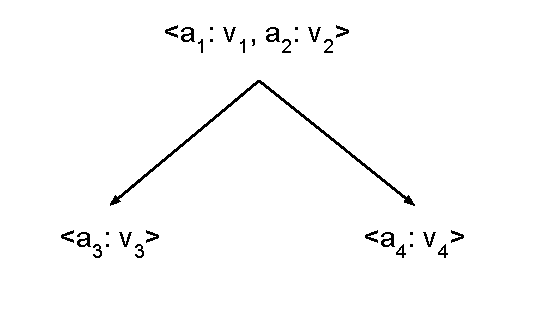
\epsfig{file=PatternExample.pdf}
\caption{An example of transaction, made of three records.}
\label{fig:transaction}
\end{figure}

Let us define a pattern.
\newdef{definition}{Definition}
\begin{definition}
A pattern is a set of ordered attributes and values belonging to possibly different records in the same transaction. In other words, a pattern is any ordered subset of $\bigcup\limits_{i=1}^{n} \bigcup\limits_{j=1}^{m} \boldsymbol{r_i}<a_j \colon v_j>$, where the ordering is given by the hierarchy of the transaction. For example, in Figure~\ref{fig:transaction} some possible example of pattern are $\{a_1 \colon v_1, a_3 \colon v_3\}$ or $\{a_2 \colon v_2, a_3 \colon v_3\}$, but not $\{a_4 \colon v_4, a_1 \colon v_1\}$, beacuse the latter breakes the hierarchic order.

A pattern has a tree structure, and it can be developed in three different ways.
\begin{itemize}
\item Horizontal -- which means that the pattern is made of a single record, with more than an attribute involved. This kind of pattern is a sort of a logical implication regarding two or more attributes in the same record, where the existence of a certain value implies the existence of some other values in the same record. Referring to Figure~\ref{fig:transaction}, the only possible horizontal pattern is $\{a_1 \colon v_1, a_2 \colon v_2\}$.
\item vertical -- when the pattern involves more than one record, and for each record one field is concerned, creating a tree structure. In this case, at least two records must be used to create such a pattern, otherwise any frequent value -- like every \texttt{tid} -- would be a pattern. The records in which appear a value belonging to the pattern do not have to be contiguous: in fact, it is possible to have a pattern made of three nodes -- for example $x, y, z$, with $x$ parent of $y$ and $y$ parent of $z$, where the existance of a value in $x$ implies the existance of a value in $z$, with any possible value in $y$. Referring to Figure~\ref{fig:transaction}, the possible vertical patterns are $\{a_1 \colon v_1, a_3 \colon v_3\}$, $\{a_2 \colon v_2, a_3 \colon v_3\}$, $\{a_1 \colon v_1, a_4 \colon v_4\}$, $\{a_2 \colon v_2, a_4 \colon v_4\}$, but also $\{a_3 \colon v_3, a_4 \colon v_4\}$. The latter is an example of a non-contiguos pattern: the parent has any value, and the two children have a value that implies the other one.
\item both horizontal and vertical -- the case of a vertical pattern, in which the records can have more than one attribute involved in the pattern. Referring to Figure~\ref{fig:transaction}, they can be $\{a_1 \colon v_1, a_2 \colon v_2, a_3 \colon v_3\}$, $\{a_1 \colon v_1, a_2 \colon v_2, a_4 \colon v_4\}$ or $\{a_1 \colon v_1, a_2 \colon v_2, a_3 \colon v_3, a_4 \colon v_4\}$.
\end{itemize}
\end{definition}

Given a set of transactions, the goal is to identify patterns of attributes that are frequent, which means transaction that appear at least a given number of time $f$.

\subsection{Big Data problem}
Starting from the data mining problem statement, the big data one is to create a set of records, which are organized in tree-structured transactions, making sure that among the transactions there exist some frequent pattern.

\section{Assumptions}
\label{sec:assumptions}
For the sake of simplification, some assumption exists.

All the records contain at least four attributes: the \texttt{rid} to identify the record; the \texttt{tid} to recognize to which transaction the record belongs; a \texttt{parent} field, containing the \texttt{rid} of the parent record -- which can be empty in case the considered record is the root of a transaction; at least another attribute, which can have any name and any type. The latter kind of attribute is called \emph{generic attribute}. The patterns are built -- and consequently searched for -- on \emph{generic attributes}, and not on the other three types, which do not create any pattern since they are used to describe the structure of the transactions.

\begin{definition}
A \emph{generic attribute} is any attribute of a record which is not the \texttt{rid}, the \texttt{tid} or the \texttt{parent} attributes. These attributes represent the features of each record, and the patterns are made of \emph{generic attributes}.
\end{definition}

All the records are assumed to have the same attributes -- some of them may be empty. Each record has discrete values, belonging to finite sets of possible values. This assumption is needed to make the data mining project easier. From the point of view of the data generation, the absence of this constraint would not complicate anything.

\section{Data generation}
\label{sec:generation}
The data generation process is parameterized, in order to let the user to use the same tool to generate various scenarios in the same problem domain. The parameters are the following:
\begin{itemize}
\item the number of transaction $T$ to be generated, which is an integer;
\item the number of patterns $P$ to generate, which are distributed among the transactions -- this is also an integer number;
\item the average length of patterns $l$, which is a floating point number;
\item the number of fields $n$ that each record has, which is an integer -- as explained in Section~\ref{sec:assumptions}, the minimum value is 4;
\item the number of values $m$ that each field can assume, which is an integer -- at least 1;
\item a threshold $t$ that indicates the number of times a pattern should appear among all transactions in order to be frequent.
\end{itemize} 
The data generation process is structured as follows: firstly, \emph{generic attributes} are generated; secondly, the patterns are generated; thirdly, the transactions are generated, including inside each of them a certain number of patterns. In the following sub-sections these three steps are explained in details.

\subsection{Attribute generation}
The very first part of the data generation process is about the attributes of the records. According to the assumptions made in Section~\ref{sec:assumptions}, each record has three attributes whose role is to uniquely identify a record -- the \texttt{rid} -- and to structure and relate records among them -- the \texttt{tid} to understand which transaction each record belongs to, and the \texttt{parent} to define the record hierarchy. In addition to these three, there is a certain number of \emph{generic attributes} that characterize each record.

All the possible \emph{generic attributes} are generated. Without loss of generality, they all are generated as strings -- since every object can be represented by a string and built from a string. In particular, $n - 3$ strings are generated, which represent the names of the attributes -- which can be also seen the keys or the field names. Then, for each attribute, a list with $m$ possible values is generated. In other words, a vector $\boldsymbol{a}$ -- of $n$ elements -- and a matrix $\boldsymbol{M}$ -- with $n$ rows and $m$ columns -- are created. The vector $\boldsymbol{a}$ contains all the attribute names, and an entry $[i, j]$ of $\boldsymbol{M}$ is the string $j$ that the attribute $i$ can assume.

To do so, let us assume the existence of a function that generates a random string, every time unique:
\begin{verbatim}
string random_string()
\end{verbatim}
which is used to generate the \emph{generic attributes}.

With the Algorithm~\ref{generate_attributes} and Algorithm~\ref{generate_values}, $\boldsymbol{a}$ and $\boldsymbol{M}$ are generated.
\begin{algorithm}
\caption{Generate the attribute names and return a vector $\boldsymbol{a}$ that contains them.}
\label{generate_attributes}
\begin{algorithmic}[1]
\Function{generateAttributeNames}{Integer $n$}
\State $\boldsymbol{a} \gets new Integer[n]$
\For{$i \gets 1 \text{ to } n$}
	\State $\boldsymbol{a}_i \gets \text{ \texttt{random\_string() }} $ 
\EndFor
\Return $\boldsymbol{a}$
\EndFunction
\end{algorithmic}
\end{algorithm}

\begin{algorithm}
\caption{Generate the attribute values and return a matrix $\boldsymbol{M}$ that contains them.}
\label{generate_values}
\begin{algorithmic}[1]
\Function{generateAttributeValues}{Integer $n$, Integer $m$}
\State $\boldsymbol{M} \gets new Integer[n][m]$
\For{$i \gets 1 \text{ to } n$}
	\For{$j \gets 1 \text{ to } m$}
		\State $\boldsymbol{M}[i, j] \gets \text{ \texttt{random\_string() }} $ 
	\EndFor
\EndFor
\Return $\boldsymbol{M}$
\EndFunction
\end{algorithmic}
\end{algorithm}

\subsection{Pattern generation}
Once the possible names and values of the fields are generated, it is the turn for the pattern to be created. To do so, let us define a tree-based data structure -- called PatternTree -- used to generate the patterns.

\begin{table}[H]
\centering
\begin{tabular}{|ll|} \hline
\textbf{PatternTree} & \\ \hline
\textbf{parent} & PatternTree \\ \hline
\textbf{children} & PatternTree[] \\ \hline
\textbf{fields} & Dict[string, string] \\
\hline\end{tabular}
\caption{PatternTree object definition.}
\label{tab:patterntree}
\end{table}

As can be seen in Table~\ref{tab:patterntree}, the object is a generic tree with an arbitrary number of children for every node. Furthermore, the attribute \emph{fields} represent the list of fields that characterize the pattern: this means that the values contained in this attribute form the pattern itself. For example, if \emph{fields} of a given node is equal to $ \{ color : blue \} $, it means that in the pattern will appear a node with the attribute \emph{color} set to \emph{blue}. The attribute \emph{fields} is a dictionary, with keys the field names, and values the field values. It does not contain the fields \texttt{rid}, \texttt{tid} and \texttt{parent}, because they are specific for a record, and not related to the pattern.

The generation of the patterns relies on four of the parameters listed at the beginning of Section~\ref{sec:generation}: the number of patterns to be generated $P$, the average length of a pattern $l$, the number of global fields $n$ and the number of values for each field $m$.

Let $Pl$ be the length of a pattern, which represents the number of edged it contains. Consequently, the number of nodes in the pattern is $1 + Pl$. The value of $Pl$ is decider using a Poisson random variable with mean $l$. This type of variable is chosen because it models events occurring successively and independently in a given time frame, and this scenario fits perfectly because the structure -- and the length -- of a single pattern is independent from the others. Furthermore, pubblications like \cite{agrawal1994fast} and \cite{ivancsy2006time} use the same approach during the pattern generation. For each node to be created, a number $k \le n$ of field names is picked randomly from the vector $\boldsymbol{a}$ generated previously, and for each field name one value is chosen from $\boldsymbol{M}$. All the nodes are saved into a set, called \emph{generated}.

Once $1 + Pl$ nodes are generated, another set is created, called \emph{included}. The latter represents the nodes exctacted from \emph{generated} to whom a parent node have been assigned. At the beginnig, this set is empty. Randomly, one node from \emph{generated} is taken and moved into \emph{included}, assigning to it a \texttt{null} parent ($\bot$ symbol): this is the root node of the pattern. 

In turn, each node in \emph{generated} is taken and moved into \emph{included}, assigning to it a parent picked from the latter set. In this way every tree takes shapes.

The Algorithm~\ref{generate_node} generates a single node, with $k \le n$ fields, while the Algorithm~\ref{generate_patterns} generates $P$ patterns, choosing the length of each one using a Poisson random variable. The latter returns a list of PatternTree object, each one is the root node of a pattern.

\begin{algorithm}
\caption{Generate a node.}
\label{generate_node}
\begin{algorithmic}[1]
\Function{generateNode}{Integer $n$, float $m$, String[] $\boldsymbol{a}$, String[][] $\boldsymbol{M}$}
\State $fields \gets \{\}$
\For{$i \gets 1 \text{ to } k$}
	\State $k \gets x : x \in [1, n]$
	\State $j \gets x : x \in [1, m]$
	\State $field\_name \gets \boldsymbol{a}_k$
	\State $field\_value \gets \boldsymbol{M}[k, j]$
	\State $fields[field\_name] \gets field\_value$
\EndFor
\State $node \gets PatternTree()$
\State $node_{fields} \gets fields$ \\
\Return $node$
\EndFunction
\end{algorithmic}
\end{algorithm}

\begin{algorithm}
\caption{Generate the patterns.}
\label{generate_patterns}
\begin{algorithmic}[1]
\Function{generatePatterns}{Integer $P$, float $l$, Integer $n$, Integer $m$, String[] $\boldsymbol{a}$, String[][] $\boldsymbol{M}$}
\State $patterns \gets \{\}$
\For{$i \gets 1 \text{ to } P$}
	\State $Pl \gets Poisson(l)$
	\State $generated \gets \{\}$
	\For{$j \gets 1 \text{ to } 1 + Pl$}
		\State $node \gets generate\_node(n, m, \boldsymbol{a}, \boldsymbol{M}) $ 
		\State $generated \gets generated \cup \{node\}$
	\EndFor
	\State $included \gets \{\}$
	\State $root \gets random\_item(generated)$
	\State $root_{parent} = \bot$
	\State $included \gets included \cup \{root\}$
	\State $generated \gets generated \setminus \{root\}$
	\For{$j \gets 1 \text{ to } 1 + Pl$}
		\State $node \gets random\_item(generated)$
		\State $parent \gets random\_item(included)$
		\State $node_{parent} = parent$
		\State $included \gets included \cup \{node\}$
		\State $generated \gets generated \setminus \{node\}$
	\EndFor
	\State $patterns \gets patterns \cup \{root\}$
\EndFor
\Return $patterns$
\EndFunction
\end{algorithmic}
\end{algorithm}

\subsection{Transaction generation}
When the patterns are generated, it is the turn for the entire transactions to be created. To do so, another data structure based on trees is defined -- called TransactionTree -- is a similar way of the one in Table~\ref{tab:patterntree}.

\begin{table}[H]
\centering
\begin{tabular}{|ll|} \hline
\textbf{TransactionTree} & \\ \hline
\textbf{parent} & TransactionTree \\ \hline
\textbf{children} & TransactionTree[] \\ \hline
\textbf{rid} & string \\ \hline
\textbf{tid} & string \\ \hline
\textbf{fields} & Dict[string, string] \\
\hline\end{tabular}
\caption{TransactionTree object definition.}
\label{tab:transactiontree}
\end{table}

The object defined in Table~\ref{tab:transactiontree} adds to each record a \texttt{rid} and the \texttt{tid}: the former is unique for each record, while the latter is unique for each transaction.

Starting from the PatternTree objects generated in the previous step, they are converted into TransactionTree objects adding them an unique \texttt{rid} and the missing fields -- those fields that will not be part of the pattern. The \texttt{tid} is not set here, it will be added later. This transformation is done in Algorithm~\ref{translate_patterns}, which is initially called passing as PatternTree $t$ the root of a pattern, and as PatternTree $p$ a \texttt{null} value $\bot$. The function transform every node of the pattern recursively.

\begin{algorithm}
\caption{Transform a PatternTree into a TransactionTree.}
\label{translate_patterns}
\begin{algorithmic}[1]
\Function{translatePatterns}{PatternTree $t$, PatternTree $p$, Integer $n$, Integer $m$, String[] $\boldsymbol{a}$, String[][] $\boldsymbol{M}$}
\State $rid \gets \text{ \texttt{random\_string() }}$
\State $fields \gets t_{fields}$
\For{$i \gets 1 \text{ to } n$}
	\If{$\boldsymbol{a}_i \notin fields$}
		\State $j \gets x : x \in [1, m]$
		\State $fields[\boldsymbol{a}_i] \gets \boldsymbol{M}[i,j]$
	\EndIf
\EndFor
\State $children \gets \{\}$
\For{$child \in t_{children}$}
	\State $children \gets children \cup \{translatePatterns(child, t, n, m, \boldsymbol{a}, \boldsymbol{M}\}$
\EndFor
\State $node \gets TransactionTree()$
\State $node_{rid} \gets rid$
\State $node_{children} \gets children$
\State $node_{fields} \gets fields$ \\
\Return $node$
\EndFunction
\end{algorithmic}
\end{algorithm}

The list of transformed pattern nodes will be referred as $TPatterns$ (Transformed patterns).

Next, a dictionary is created to determine in which transactions each pattern in $TPatterns$ will appear. The dictionary uses the elements of $TPatterns$ as keys, and integer lists as values. The integer lists contain the indexes of the transactions in which the pattern (its key) needs to be present. For example, if the algorithm is generating transaction number $k$ and the integer lists associated with patterns $P1$ and $P2$ contain $k$, then both $P1$ and $P2$ will be appended into transaction $k$. The number of transactions in which each pattern will appear is determined by the pattern size, meaning that shorter patterns will appear more often compared to bigger patterns. Furthermore, by definition, the patterns should be frequent, thus a minimum number of transactions in which each pattern will appear is guaranteed. The minimum frequency is determined by paramater $t$. Once the number of times each pattern should appear over all transactions is determined, the actual transactions in which each of them will appear are chosen randomly, meaning that a pattern may appear more than one time in a given transaction. Algorithm~\ref{generate_indexes} shows the exact procedure and formulas used to generate the pattern appearance dictionary. Line 5 shows the formula used to compute the number of time a given pattern should appear among all transactions where $min\_nodes$ stands for the number of nodes in the smallest pattern, $max\_nodes$ stands for the number of nodes in the biggest pattern. Both of these values are computed by searching for the biggest and the smallest pattern in $TPatterns$.
\begin{algorithm}
\caption{Generate transaction indexes for all patterns.}
\label{generate_indexes}
\begin{algorithmic}[1]
\Function{GenerateIndexesDictionary}{TransactionTree[] $TPatterns$, Integer $max\_nodes$, Integer $min\_nodes$, Integer $T$, Integer $t$}
\State $transaction\_indexes \gets \{\}$
\ForEach{$pattern \in TPatterns$}
	\State $indexes \gets [\:]$
	\State $k \gets T - (|pattern| - min\_pattern\_nodes) \times (T - t) / (max(1, max\_pattern\_nodes - min\_pattern\_nodes))$
	\For{$i \gets 0 \text{ to } k - 1$}
	\State $indexes[i] \gets random\_int(0, T - 1)$
	\EndFor
	\State $transaction\_indexes[pattern] \gets tree\_indexes$
\EndFor
\Return $transaction\_indexes$
\EndFunction
\end{algorithmic}
\end{algorithm}

To better understand how this formula allows to determine the number of indexes to generate, let's suppose that we want to compute the number of indexes for a pattern with 2 nodes, a pattern with 4 and a pattern with 6. Let's also suppose that the total number of transaction $T$ equals 100, that the minimum appearance threshold $t$ equals 20 and that the computed values for $min\_nodes$ and $max\_nodes$ are 2 and 6 respectively. The number of appearances for the first pattern $k$ is going to be computed as (100 - (2 - 2) * (100 - 20) / (max(1, 6 - 2))). As we can notice, since the pattern is the smallest it can be, the whole right side of the formula is going to equal 0 because of the first expression (2 - 2) consequently, $k$ is going to equal $T$. This makes sense as the pattern is the smallest it could be and it should appear a number of times equals to the total transactions. Notice that this does not mean that this pattern is going to appear in every transaction as the indexes are generated randomly and it may well be that the same index is generated more than once. For the second pattern the formula is going to be computed as (100 - (4 - 2) * (100 - 20) / (max(1, 6 - 2))). This time the right side of the expression is going to be equal to 40 and $k$ is going to equal $T$ - 40. This makes sense as the second pattern is twice as big compared to the first one and it should appear fewer times. For the last pattern the formula is going to be computed as (100 - (6 - 2) * (100 - 20) / (max(1, 6 - 2))). This time the right side of the expression is going to be equal to 80 and $k$ is going to equal $t$. Since the last pattern is the biggest, it makes sense for it to appear only the minimum number of times to make it frequent.

To sum it up, the formula makes so that the smallest patterns appear as many times as there are transactions, the biggest patterns appear just enough times to be frequent, and all the patterns in between appear in intermediate number of times between these two values.

Finally, the actual transactions are generated and this sequence of steps is repeated for each transaction: Firstly, a pattern list is created, and all the patterns which contains the transaction index in their index list generated with Algorithm~\ref{generate_indexes} are appended to it. This list will be named $chosen\_patterns$ and the above described process can be seen in Algorithm \ref{pick_patterns}.


\begin{algorithm}
\caption{Pick the patterns for the current transaction being generated}
\label{pick_patterns}
\begin{algorithmic}[1]
\Function{PickPattern}{TransactionTree[] $TPatterns$, Dict(TransactionTree, Integer) $transaction\_indexes$, Integer $current\_transaction\_index$}
\State $chosen\_patterns \gets []$
\State $chosen\_pattern\_index \gets 0$
\ForEach{$pattern \in TPatterns$}
    \For{$i \gets 0 \text{ to } |transaction\_indexes[pattern]| - 1$}
        \If{$transaction\_indexes[pattern][i] = current\_transaction\_index$}
            \State $chosen\_patterns[chosen\_pattern\_index] \gets pattern$
            \State $chosen\_pattern\_index \gets chosen\_pattern\_index + 1$
        \EndIf
    \EndFor
\EndFor
\Return $chosen\_patterns$
\EndFunction
\end{algorithmic}
\end{algorithm}

Secondly, some $TransactionTree$ nodes are generated each with $n$ - 3 randomly generated attributes, plus a unique \texttt{rid} field. The number of generated nodes depends on the size of $chosen\_pattern$ list and on the $l$ parameter. These nodes serve the only purpose of adding random nodes to the transactions. The fields and values for these nodes are picked at random from the previously generated $\boldsymbol{a}$ vector and $\boldsymbol{M}$ matrix. This process is described in Algorithm \ref{generate_random_nodes}.

\begin{algorithm}
\caption{Generate the random nodes to be appended to the current transaction being generated}
\label{generate_random_nodes}
\begin{algorithmic}[1]
\Function{GenerateRandomNodes}{TransactionTree[] $chosen\_patterns$, float $l$, String[] $a$, String[][] $M$}
\State $random\_nodes \gets []$
\For{$i \gets 0 \text{ to } 1 + l + l \times |chose\_patterns|$}
    \State $rid \gets \text{ \texttt{random\_string() }}$
    \State $fields\_for\_record \gets \{"rid": rid, "parent": None\}$
    \For{$j \gets 0 \text{ to } |a| - 1$}
        \State $field\_value \gets M[j][random\_int(0, |M[j]| - 1)]$
        \State $fields\_for\_record[a[j]] \gets field\_value$
    \EndFor
    \State $random\_nodes[i] \gets TransactionTree()$
    \State $random\_nodes_{fields} \gets fields\_for\_record$
\EndFor
\Return $random\_nodes$
\EndFunction
\end{algorithmic}
\end{algorithm}

Thirdly, the randomly generated nodes and the $chosen\_patterns$ elements are merged together into one list which will be called $nodes\_to\_append$, and an unique \texttt{tid} is assigned to each member of this list. A root for the transaction is then chosen randomly from $nodes\_to\_append$. This process can be seen in Algorithm \ref{merging_lists} and Algorithm \ref{transaction_generation}.

\begin{algorithm}
\caption{Merging of the two lists and assignment of the tid}
\label{merging_lists}
\begin{algorithmic}[1]
\Function{MergeLists}{TransactionTree[] $chosen\_patterns$, TransactionTree[] $random\_nodes$}
\State $transaction\_id = \text{ \texttt{random\_string() }}$
\State $complete\_nodes\_list \gets []$
\For{$i \gets 0 \text{ to } |chosen\_patterns| - 1$}
    \State $chosen\_patterns[i]_{fields}["tid"] \gets transaction\_id$
    \State $complete\_nodes\_list[i] \gets chosen\_patterns[i]$
\EndFor
\State $k \gets |chosen\_patterns|$
\For{$i \gets k \text{ to } k + |random\_nodes| - 1$}
    \State $random\_nodes[i - k]_{fields}["tid"] \gets transaction\_id$
    \State $complete\_nodes\_list[i] \gets random\_nodes[i - k]$
\EndFor
\Return $complete\_nodes\_list$
\EndFunction
\end{algorithmic}
\end{algorithm}

Furthermore, another list called $current\_tree$ is created, and its purpose is to store the nodes which are already part of the transaction; the root node, together with all the pattern nodes if a pattern was chosen as root, is appended to this list.

Fourthly, as long as there are elements in the $nodes\_to\_append$ list, the algorithm will keep choosing random nodes from it and append them to nodes in the $current\_tree$ list randomly. When a node is appended to the tree, it is deleted from the $nodes\_tp\_append$ list and inserted into the $current\_tree$ list, together with all the pattern nodes if the appended node is a pattern root. Once the $nodes\_to\_append$ list is empty, the transaction root is appended to the return array. This process is shown in Algorithm \ref{transaction_generation}. To sum it up, for each transaction to be generated function PickPattern (Algorithm \ref{pick_patterns}) is called to select the patterns that should appear in the transaction. Next, a number of random nodes to be appended to the transaction is generated using the GenerateRandomeNodes function (Algorithm \ref{generate_random_nodes}). Next, using the function MergeLists (Algorithm \ref{merging_lists}), the chosen patterns and the randomly generated nodes are merged into one list and a transaction id is assigned to all the nodes in this list. Finally, the function SingleTransactionGeneration (Algorithm \ref{transaction_generation}) is called to randomly append all the nodes in order to generate the transaction. This whole process is shown in Algorithm \ref{complete_transaction_generation}.

\begin{algorithm}
\caption{Generation of single transaction}
\label{transaction_generation}
\begin{algorithmic}[1]
\Function{SingleTransactionGeneration}{TransactionTree[] $complete\_nodes\_list$, TransactionTree[] $chosen\_patterns$}
\State $transaction\_root \gets complete\_nodes\_list[random\_int(0, |complete\_nodes\_list| - 1)]$
\State $current\_tree \gets [transaction\_root]$
\State $current\_tree\_index \gets 1$
\If{$transaction\_root \in chosen\_patterns$}
    \ForEach{$node \in transaction\_root.getNodes()$}
        \State $current\_tree[current\_tree\_index] \gets node$
        \State $current\_tree\_index \gets current\_tree\_index + 1$
    \EndFor
\EndIf
\State $complete\_nodes\_list.remove(transaction\_root)$
\For{$i \gets 0 \text{ to } |complete\_nodes\_list| - 1$}
    \State $node\_to\_append \gets complete\_nodes\_list[random\_int(0, |complete\_nodes\_list| - 1)]$
    \State $chosen\_parent \gets current\_tree[random.int(0, |current\_tree| - 1)]$
    \State $chosen\_parent.addChild(node\_to\_append)$
    \State $current\_tree[current\_tree\_index] \gets node\_to\_append$
    \State $current\_tree\_index \gets current\_tree\_index + 1$
    \If{$node\_to\_append \in chosen\_patterns$}
        \ForEach{$node \in node\_to\_append.getNodes()$}
            \State $current\_tree[current\_tree\_index] \gets node$
            \State $urrent\_tree\_index \gets urrent\_tree\_index + 1$
        \EndFor
    \EndIf
    \State $complete\_nodes\_list.remove(node\_to\_append)$
\EndFor
\Return $transaction\_root$
\EndFunction
\end{algorithmic}
\end{algorithm}

\begin{algorithm}
\caption{Generation of all transactions}
\label{complete_transaction_generation}
\begin{algorithmic}[1]
\Function{TransactionGeneration}{TransactionTree[] $TPatterns$, Integer $T$, float $l$, String[] $a$, String[][] $M$, Dict(TransactionTree, Integer) $transaction\_indexes$}
\State $root\_list \gets []$
\State $root\_list\_index \gets 0$
\For{$index \gets 0 \text{ to } T - 1$}
    \State $chosen\_patterns \gets \text{PickPattern(TPatterns, transaction\_indexes, index)}$
    \State $random\_nodes \gets \text{GenerateRandomNodes(chosen\_patterns, l, a, M)}$
    \State $complete\_nodes\_list \gets \text{MergeLists(chosen\_patterns, random\_nodes)}$
    \State $transaction\_root \gets \text{SingleTransactionGeneration(complete\_nodes\_list, chosen\_patterns)}$
    \State $root\_list[root\_list\_index] \gets transaction\_root$
    \State $root\_list\_index \gets root\_list\_index + 1$
\EndFor
\Return $root\_list$
\EndFunction
\end{algorithmic}
\end{algorithm}

\section{Implementation}
The various steps and algorithms explained in Section~\ref{sec:generation} are implemented in a program, that takes as input the parameters listed in the previous section, and it produces a set of records organized in transactions, saving the generated data into a \texttt{csv} file. The latter has $n + 1$ rows, where the first line lists the names of the fields present inside each record, and the following $n$ lines contains the value of the fields, one record per line.

The software is written in Python\footnote{www.python.org}, and it makes use of the Numpy\footnote{http://www.numpy.org/} library \cite{oliphant2006guide} for manipulating arrays and matrices. The parameters are passed as arguments with flags and values when the program is started. The user can specify her own parameters, or use the default ones. It is also possible to set a flag to let the program print on the standard output which are the generated pattern. In this way is easy to test the correctness of the miner software that searches for these patterns.

\subsection{Use the software}
To use the software, is necessary to have a Python interpreter, at least at version 3.6, and to install the dependencies -- the libraries needed by the software -- running the command \texttt{pip install -r requirements.txt}. To launch the software is necessary to run the command \texttt{python src/main.py <arguments>}, with the following possible argument list:
\begin{itemize}
\item \texttt{-out filename}, to specify the filename on which the output is written. Default is \texttt{output}. Note that the extension \texttt{.csv} is automatically added, so passing the value \texttt{output} will produce a file named \texttt{output.csv};
\item \texttt{-t 10}, to specify how many transaction to generate. Default is 20;
\item \texttt{-p 10}, number of patterns to create. Default is 4;
\item \texttt{-avg 10}, the average length of a pattern. Default is 3;
\item \texttt{-nf 10}, the number of fields each records will have. Default is 10;
\item \texttt{-nv 10}, the number of values each field can assume. Default is 100;
\item \texttt{-avg 10}, the average length of a pattern. Default is 3;
\item \texttt{-thr 3}, the minimum number of times a pattern appears. Default is 4;
\item \texttt{-pp true}, to print on the standard output the generated patterns. Default is false;
\end{itemize}

\section{Evaluation}
The software is developed using an object oriented paradigm, and therefore it is composed by many small components that interact with each other. Each of this component has been tested, with several test cases, to verify its behaviour and its correctness.

In addition to that, some other tests have been performed, focused on the scalability. Since the application requires many parameters to work, some of them are kept constant in every test, like the maximum number of attributes a record can have $n$, the number of possible values each field can assume $m$, the average pattern length $l$ and the threshold $t$ that indicates how many times a pattern has to appear to be considered frequent. In particular, the following value are used: $n = 10, m = 100, l = 5.0, t = 5$. Then, fixed the number of pattern $P$ to generate, our tests iterate on a list of integer, that represent the number of transaction $T$ to generate. The software is launched with these parameters, and the response time is saved and plotted with respect to $T$. For each test, the value of $T$ that are used are 10, 20, 50, 100, 200, 500, 1000. For each configuration, 5 tests are performed.

\begin{figure}
\centering
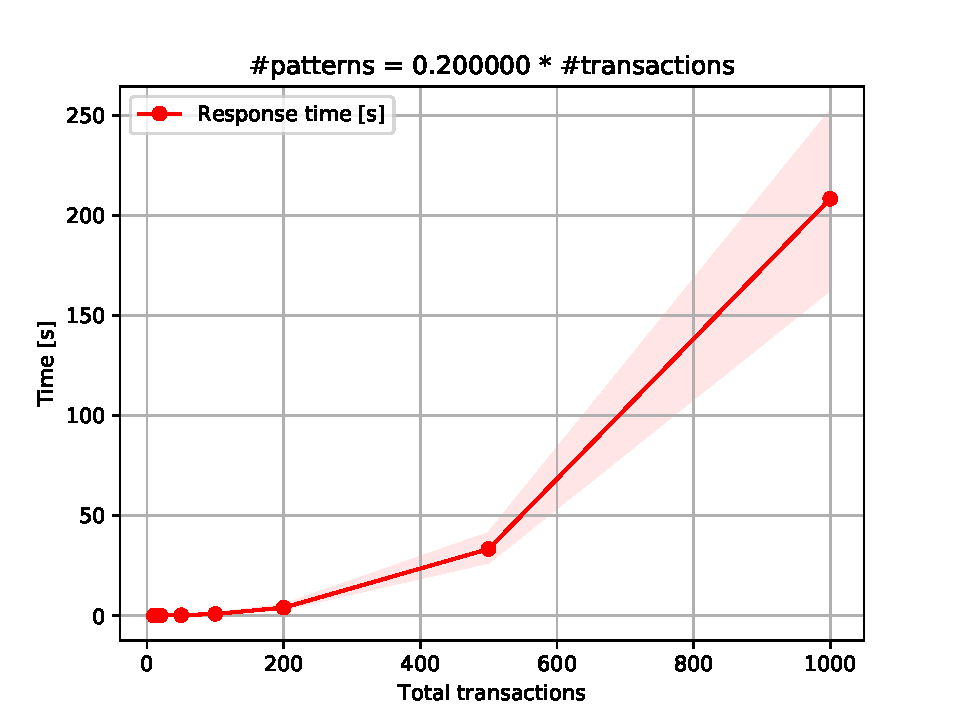
\epsfig{file=t02.pdf, scale=0.5}
\caption{Test results with $P = 0.2 * T$.}
\label{fig:zerotwo}
\end{figure}

\begin{figure}
\centering
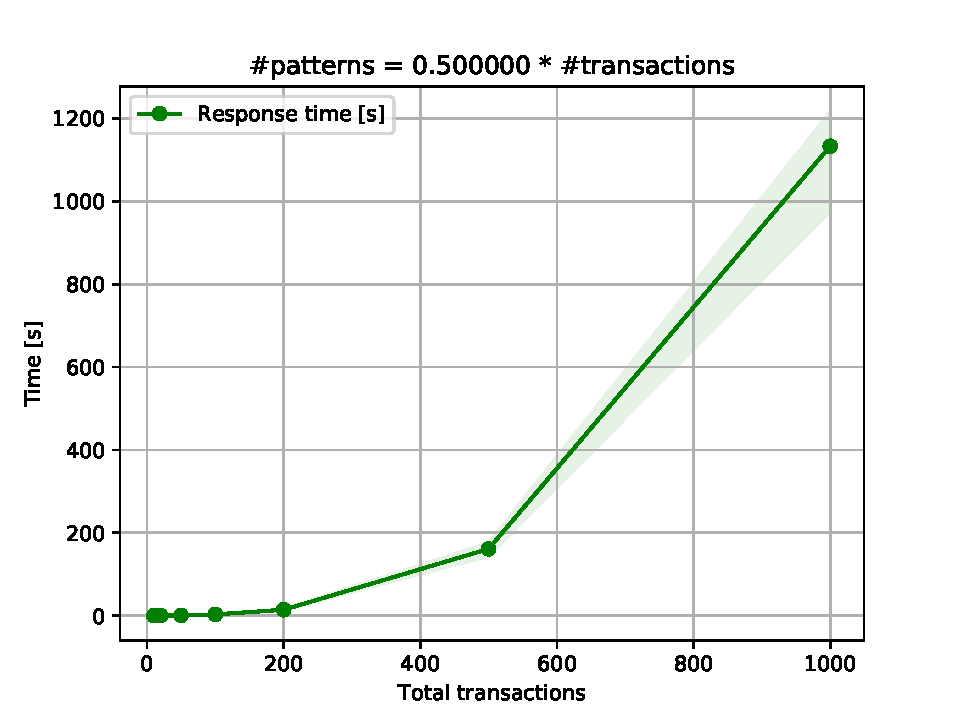
\epsfig{file=t05.pdf, scale=0.5}
\caption{Test results with $P = 0.5 * T$.}
\label{fig:zerofive}
\end{figure}

\begin{figure}
\centering
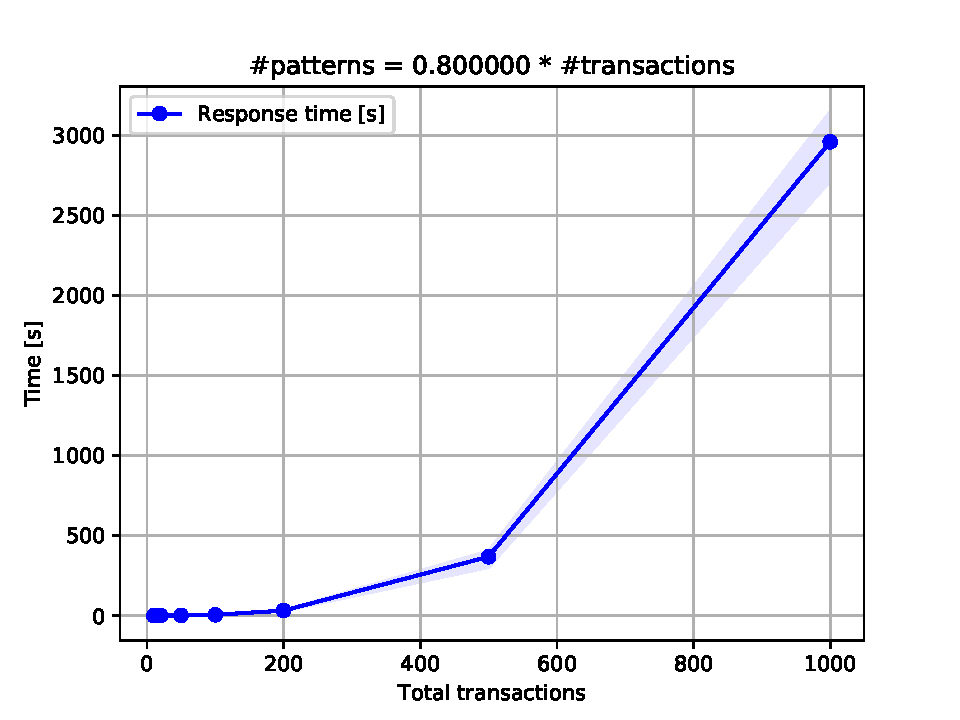
\epsfig{file=t08.pdf, scale=0.5}
\caption{Test results with $P = 0.5 * T$.}
\label{fig:zeroeight}
\end{figure}

\begin{figure}
\centering
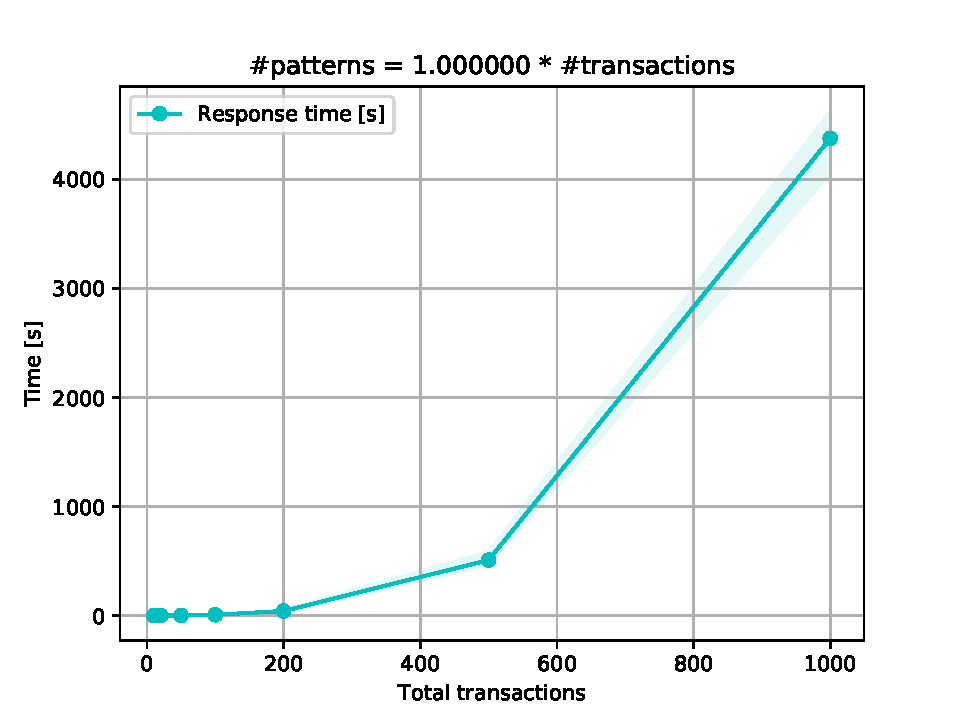
\epsfig{file=t1.pdf, scale=0.5}
\caption{Test results with $P = T$.}
\label{fig:one}
\end{figure}

The Figure~\ref{fig:zerotwo} shows the performances of the software with a fixed value of patterns to generate $P = 0.2 * T$, the Figure~\ref{fig:zerofive} with $P = 0.5 * T$, the Figure~\ref{fig:zeroeight} with $P = 0.8 * T$, and the Figure~\ref{fig:one} with $P = T$. Each of them plots the average response time of each configuration of the tests, but also the region between the minimum and the maximum time taken to repond for each configuration is colored, to show a best and a worst case.

As can be seen, the parameter $P$ plays an important role in the outcomes, since the higher it is, the higher the total time. The shapes of the four graphics are the same, but with different scales, because of $P$. The test are performed on a machine with a 2.7 Ghz Intel Core i7 processor, and 16 GB of RAM.

\section{Conclusions}
In this report is described the used methods, the algorithms and the results obtained during the implementation of a parameterized generator for frequent item sets mining in tree-like sequences of complex objects. Python is used to implement a generator which adjusts its outcome based on parameters such as pattern average length to vary the size of the patterns, pattern number to vary the number of patterns which can appear and pattern frequency to vary the minimum frequency that a pattern must have. Finally, the behaviour of the software is tested as its input increases. Of course, both the randomness with which data is generated, and the respect of the given parameters may lead to very long executions, but on the other hand the outcome contains unbiased and complete results, with pattern of different nature, structure and distribution.

\subsection{Future works}
It is possible to work on the performances of the software, trying to parallelize as much as possible the process of generating data. In fact, once the name of the fields $\boldsymbol{a}$ and the values of the attributes $\boldsymbol{M}$ are generated, it would be feasible to assign the generation of a single pattern to a specific thread. Since they would just read from $\boldsymbol{a}$ and $\boldsymbol{M}$, any synchronization protocol would not be needed in this phase.

In parallel, some other threads might start to generate the real patterns, with random length and random contents. Once all the patterns are generated, each thread would take in charge the pattern generated by itself and it would append it to some transaction. In this phase some synchronization procedures would be necessary, since a transaction can contain more than one pattern, and therefore more than one thread would try to concurrently modify a single transaction.

This approach should be effective specially with multi processors machines, like a server.


\bibliographystyle{abbrv}
\bibliography{sigproc}  % sigproc.bib is the name of the Bibliography in this case

\end{document}
